%! Author = weiss
%! Date = 20.01.2025
\Author{\daAuthorThree}
    This chapter concentrates on exploring the Spring ecosystem and covers core components like Spring Framework, Spring Boot and Spring Data JPA. It highlights the advantages of this ecosystem in simplifying Java development and improving the efficiency.

    \subsection{Spring Boot}
    Spring Boot is a tool which makes developing web applications and microservices with the Java Spring Framework faster and easier. As powerful as the Spring Framework on its own is, it still requires much time and knowledge to configure, set-up and deploy Spring apps. Spring Boot tries to mitigate this effort with three features 

    \textbf{Autoconfigure:}
        \begin{itemize}
            \item Autoconfigure initializes Spring apps with a preset of dependencies so that the developer does not have to configure those manually. Spring Boot comes with this feature to automatically configure the Spring Framework and third-party packages based on your needs for the project. Even though you can override the default configuration
            after the initialization, the initial setup makes the development process faster and more efficient. Meanwhile the autoconfiguration also reduces the possibility of many human errors which can occur during the configuration of an Java application.
        \end{itemize}
    \textbf{Opinionated Approach:}
        \begin{itemize}
            \item Spring Boot uses an opiniated approach while adding and configuring the starter dependencies which is based on the needs of the project. Rather than requiring you to make all the decisions yourself and setup everything manually, Spring Boot uses its own common sense to choose which packages to install and which default values to use.
            During the initialization, you can define the needs and requirements of your project. Throughout this process you can choose from a huge collection of starter dependencies which are called "Spring Starters" that cover every day use cases.
            To give an example, the "Spring Web" dependency simplifies building Spring-based web apps which require minimal configuration work by adding all the other necessary dependencies that you may need for creating such an app. "Spring Security" is another popular starter dependency which automatically adds authentication and access-control
            features to an application.
            Spring Boot on its own includes over 50 Spring Starters. However there are many more third-party starters that are also available.
        \end{itemize}
    \textbf{Stand-Alone Application:}
        \begin{itemize}
            \item Spring Boot also helps developers create apps that just run. What that means is that you can create stand-alone applications that run on their own without needing any external web servers.
            This can be done by including(/embedding) a web server such as Tomcat into your app during the initialization process. As a consequence of this you can start your app on any platform by using the command to run the app.
        \end{itemize}                
    
    \textbf{Setting up a Spring Boot app:} \newline
    You can easily setup a Spring Boot project using the \textbf{Spring Initializr}. If you want to create your own Spring Boot-based project, you can just visit the \textbf{Spring Initializr}, fill in your project details and download a bundled up project as a .zip file. During the initialization process you have to choose a couple of factors that impact the structure of the 
    project such as the programming language, the Spring Boot version and of course any other dependency you may need to make the development easier and more efficient.
    Depending on the IDE (vergiss net des zu includen am ende) you use to develop the app, you maybe able to create a Spring Boot project in the IDE itself. Creating a new Spring Boot project in the IDE gives you the same options to choose to make your life easier while developing the app. However, not all IDEs support creating such a project
    on their own, so you may need to install a addon to create a Spring Boot project.

    \begin{figure} [H]
        \centering
        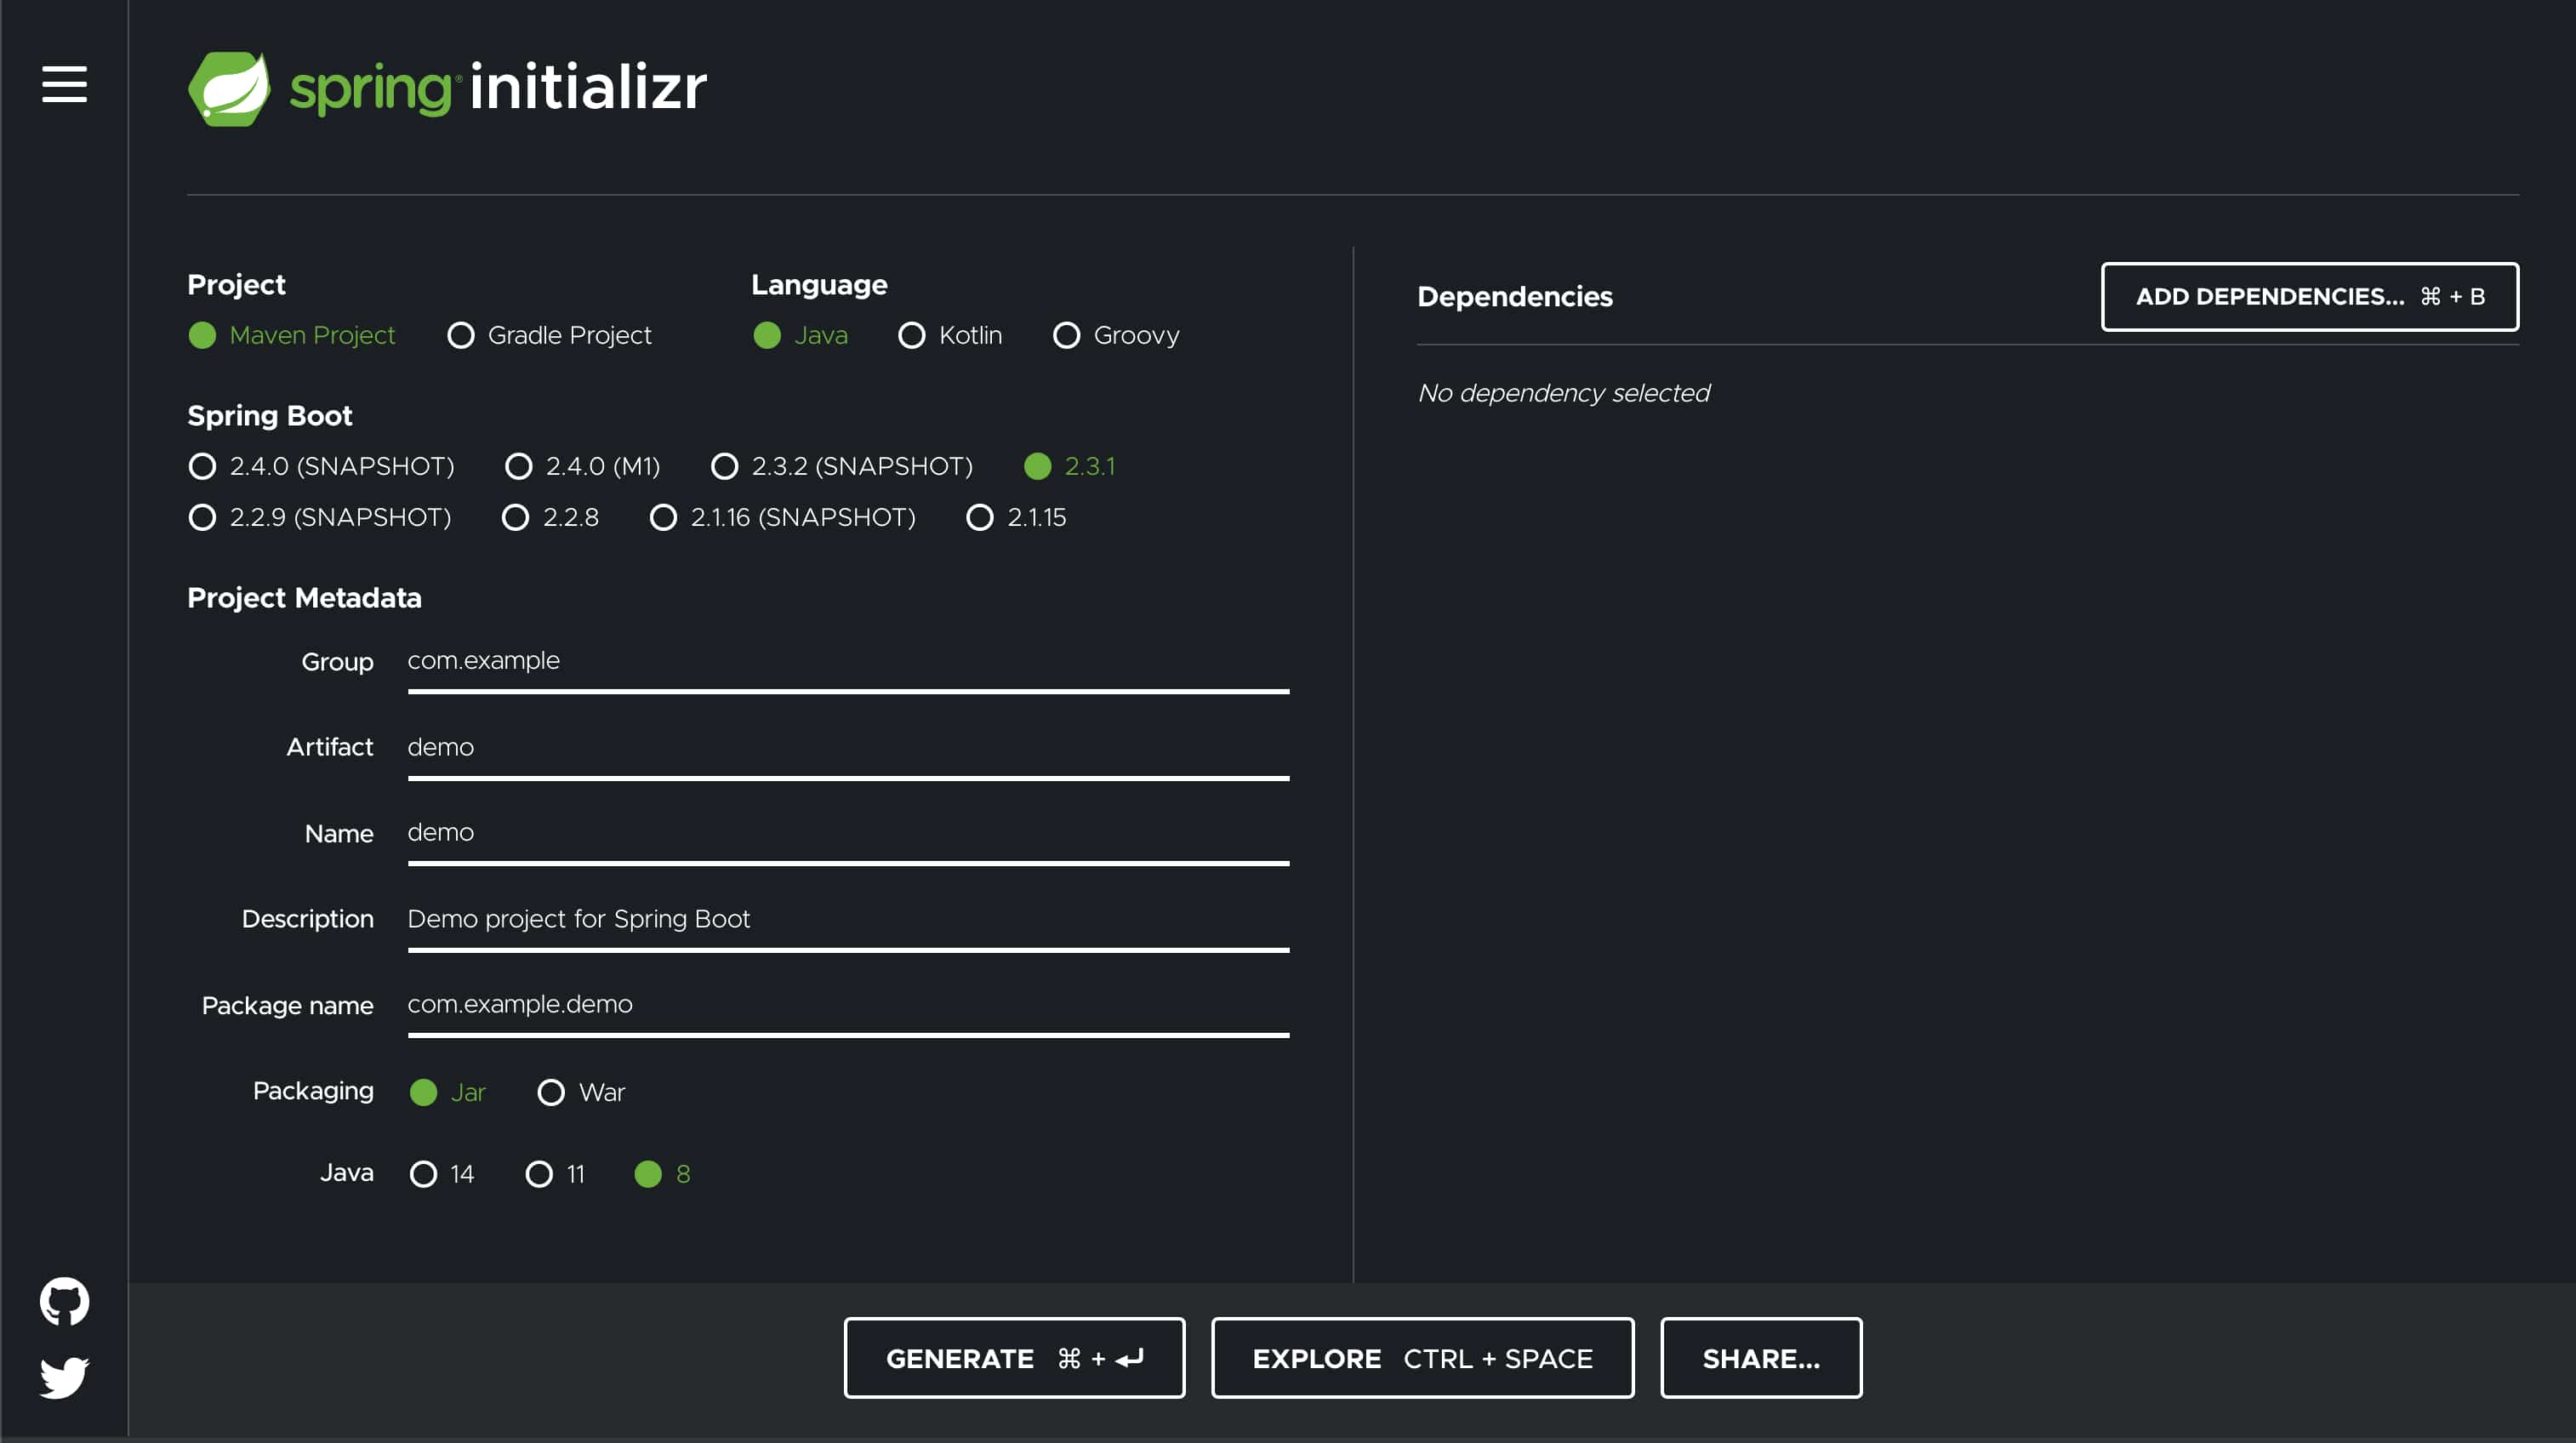
\includegraphics [width=1\textwidth] {images/andreas/springFramework/springInit.jpg}
        \caption{GUI of the Spring Initializr}
    \end{figure}
    
    \textbf{Difference between Spring Boot and Spring Framework:} \newline
    The biggest advantages of using Spring Boot and not Spring alone are the easier use and faster development. Theoretically, this advantage of Spring Boot comes at the cost of the greater flexibility you would get from working directly wit Spring Framework. However, in practice, using Spring Boot is worth the trade because you are still able to use
    Spring Framework's annotation system to inject extra dependencies more easily into you app. Furthermore you still get access to all of Spring Framework's features which include easy event handling and built-in security. 
    
    \subsection{Spring Data JPA}
    Spring Data JPA stands for Java Persistence API and provides a specification for persisting, reading and managing data from the object in your program, which are called entities, to your tables in the database. JPA specifies a set of rules for developing interfaces that follow specific standards. As a result, JPA is just some guidelines to implement ORM.
    ORM is the process of persisting an object in java directly into a database table. \newline
    The goal of Spring Data JPA is to create classes called "Repositories" which significantly reduce the amount of unnecessary code to access and manipulate data from the database of your project. \newline
    \textbf{Entities:} \newline
    As already mentioned, the object from which Spring Data JPA manages the data are called entities. Every table of your database is an entity with each attribute being a column in the respective table. You can use the \texttt{@Entity} annotation in your code to specify that said class is an entity and needs to be in the database. However, this annotation is not
    the only one which is supported by JPA. Using annotations such as \texttt{@Id} or \texttt{@GeneratedValue}, you can define different features of your entity and therefore your table in the database. Those annotations are a way to make the development of the project much faster and even more efficient. \newline
    \textbf{Data access object layer:} \newline
    Although there are many annotations that are usable for your entity, there is one annotation which is a core feature in JPA. The \texttt{@Repository} annotation is a marker for a class that fulfills the role of a repository which is also know as a Data Access Object. However, something else need to be done when using the \texttt{@Repository} annotation. If you use
    this annotation, you also need to extend your repository class with the JpaRepository-class which implements many methods to manage, manipulate and sort or filter all the data in any Table of the Database. You can too make custom queries in your repository class if the operation you need is not available by standard. \newline
    \textbf{Service Layer:} \newline
    Classes that use the \texttt{@Service} annotation are used with classes that provide some data manipulation methods such as a repository-class. By implementing such a class, the project structure is better understandable and more clear to other developers which may work on this project later on.  \newline
    \textbf{Controller Layer:} \newline
    This Layer provides the applications with the routes with which the data can get manipulated through a GUI. With the \texttt{@RestController} annotation, you can declare a class as an actual controller. The controller uses the service classes from the service layer to get the data or manipulate it in any way. It also specifies the routes which you can then
    access in any form of user interface so that the user can actually use or see the data. \newline
    \textbf{Mappings:} \newline
    There are some annotations which defines the routes with all its features and where you can access the route. The \texttt{@GetMapping} gives the user data in any form. This can be all the data from a table or a specific entry in a table based on any filter. The \texttt{@PostMapping} is used if a user would want to create a new entry in a specific table. 
    For example if you have a management program in your company, you may want to add an employee and this annotation is used to create the route which can then be used by the manager to add a new employee to the database. If, for example, the address or surname of this employee would change, you would need the \texttt{@PutMapping} to update
    the data stored for this employee in the database. However, if this said employee would resign from your company, then you would need the \texttt{@DeleteMapping} annotation for the manager to be able to clear this employee out of the company's database.
    Now you can access all those routes through your graphical interface to show the user the data they can and need to access, manage or even delete.
    
    \subsection{Lombok} \todo{ich würde gern mehr über Lombok schreiben weiß aber net genau was noch, bitte vorschläge} \newline
    In the modern days of Java development, one big challenge developers face is writing boilerplate code which are code segments that repeat itself over and over again and get used often in a project. This is especially the case in frameworks like Spring Boot where we use classes like the service layer that involve a significant amount of repetitive code.
    "Project Lombok" is a Java libtary that has the aim to reduce this boilerplate code by automatically generating the code for commonly used patterns. By integrating Lombok in your Spring Boot project, you can not only simplify your code but make it easier to read maintain and write. 
    Lombok works great with the whole Spring framework. If you would want to use a project with Spring Data JPA, you would not get that far without using any annotations provided by Project Lombok. To flag an entity class for Spring Data JPA, you need to use the \texttt{@Entity} annotation. This annotation comes from the Lombok library and adds a couple of 
    features to this class so that JPA recognizes it as an entity for the database.

    \subsection{Spring Security}
    this is where the Spring Security part is but i have to do it first so pls this part has to chill now
    
    \subsection{Advantages}
    Now in retrospect, what are the advantages by/with using the Spring Framework and why did we choose it for our backend.
    Reduced Boilerplate Code: A huge factor of the Spring framework is its abilty to reduce repetitive code segments. Mainly through the Lombok library, the Spring framework gives the developer many ways to exchange repetitive code with annotations. \newline 
    \textbf{Enhanced Testability:} \newline
    With Spring's huge library of dependencies you can not only get dependencies which make the coding easier but the testing too. Some dependencies gave us mock data to test the backend endpoints easier.\newline
    \textbf{Flexibility:} \newline
    The same thing that helped us testing, gave us and other projects the flexibility with which you can for example expand or change certain things in your project. This was extremely helpful for us because a certain requirement changed while we were developing the backend.\newline
    \textbf{Consistency:} \newline
    Spring provides consistent programming and configurations models across many different types of applications. Whether you would want to develop a web application or a microservice, Spring offers a unified approach which improves developer productivity.\newline
    \textbf{Improved Productivity:} \newline
    Tools like Spring Boot, which are part of the Spring ecosystem, significantly enhance developer productivity by providing better approaches to different problems and embedded servers.\newline 
    